% This file was created by matlab2tikz.
%
%The latest updates can be retrieved from
%  http://www.mathworks.com/matlabcentral/fileexchange/22022-matlab2tikz-matlab2tikz
%where you can also make suggestions and rate matlab2tikz.
%
\definecolor{mycolor1}{rgb}{0.00000,0.44700,0.74100}%
%
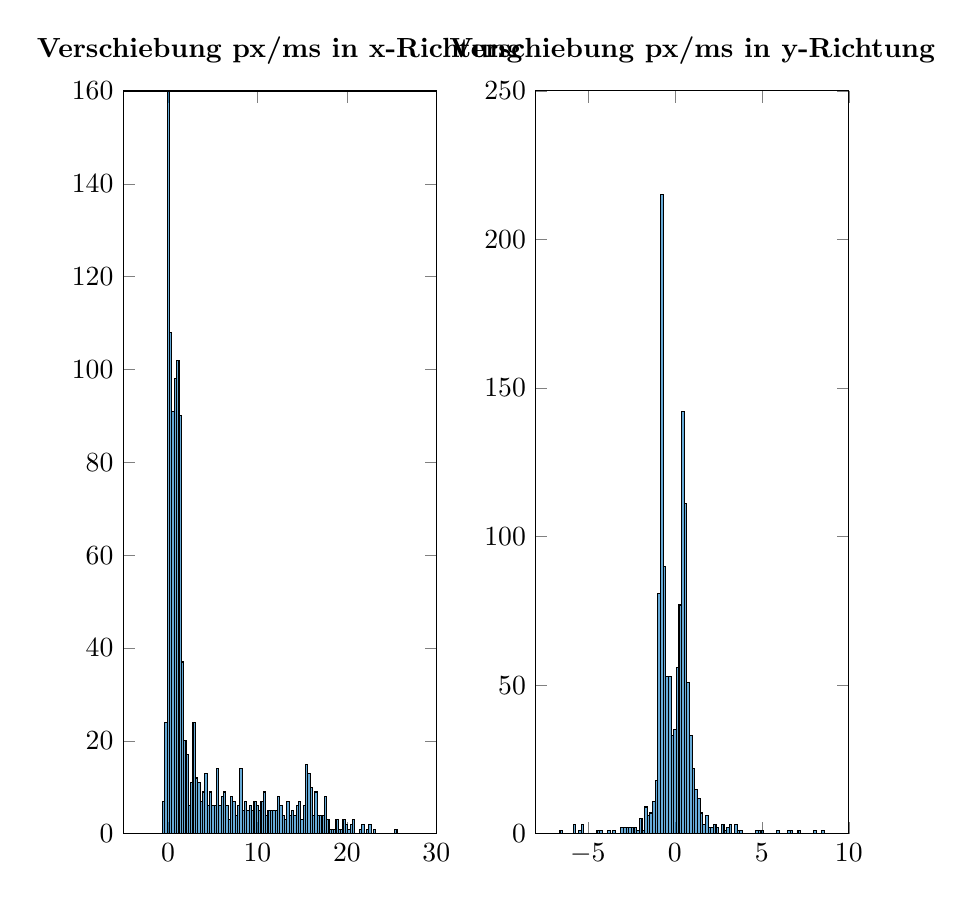
\begin{tikzpicture}

\begin{axis}[%
width=0.328\textwidth,
height=0.778\textwidth,
at={(0\textwidth,0\textwidth)},
scale only axis,
xmin=-5,
xmax=30,
ymin=0,
ymax=160,
axis background/.style={fill=white},
title style={font=\bfseries},
title={Verschiebung px/ms in x-Richtung}
]
\addplot[fill=mycolor1,fill opacity=0.6,draw=black,ybar interval,area legend] plot table[row sep=crcr] {%
x	y\\
-0.6	7\\
-0.338	24\\
-0.0760000000000001	160\\
0.186	108\\
0.448	91\\
0.71	98\\
0.972	102\\
1.234	90\\
1.496	37\\
1.758	20\\
2.02	17\\
2.282	6\\
2.544	11\\
2.806	24\\
3.068	12\\
3.33	11\\
3.592	7\\
3.854	9\\
4.116	13\\
4.378	6\\
4.64	9\\
4.902	6\\
5.164	6\\
5.426	14\\
5.688	6\\
5.95	8\\
6.212	9\\
6.474	6\\
6.736	3\\
6.998	8\\
7.26	7\\
7.522	4\\
7.784	6\\
8.046	14\\
8.308	5\\
8.57	7\\
8.832	5\\
9.094	6\\
9.356	5\\
9.618	7\\
9.88	6\\
10.142	5\\
10.404	7\\
10.666	9\\
10.928	4\\
11.19	5\\
11.452	5\\
11.714	5\\
11.976	5\\
12.238	8\\
12.5	6\\
12.762	4\\
13.024	3\\
13.286	7\\
13.548	4\\
13.81	5\\
14.072	4\\
14.334	6\\
14.596	7\\
14.858	3\\
15.12	6\\
15.382	15\\
15.644	13\\
15.906	10\\
16.168	4\\
16.43	9\\
16.692	4\\
16.954	4\\
17.216	4\\
17.478	8\\
17.74	3\\
18.002	1\\
18.264	1\\
18.526	1\\
18.788	3\\
19.05	1\\
19.312	1\\
19.574	3\\
19.836	2\\
20.098	1\\
20.36	2\\
20.622	3\\
20.884	0\\
21.146	0\\
21.408	1\\
21.67	2\\
21.932	0\\
22.194	1\\
22.456	2\\
22.718	0\\
22.98	1\\
23.242	0\\
23.504	0\\
23.766	0\\
24.028	0\\
24.29	0\\
24.552	0\\
24.814	0\\
25.076	0\\
25.338	1\\
25.6	1\\
};
\end{axis}

\begin{axis}[%
width=0.328\textwidth,
height=0.778\textwidth,
at={(0.432\textwidth,0\textwidth)},
scale only axis,
xmin=-8,
xmax=10,
ymin=0,
ymax=250,
axis background/.style={fill=white},
title style={font=\bfseries},
title={Verschiebung px/ms in y-Richtung}
]
\addplot[fill=mycolor1,fill opacity=0.6,draw=black,ybar interval,area legend] plot table[row sep=crcr] {%
x	y\\
-6.6	1\\
-6.448	0\\
-6.296	0\\
-6.144	0\\
-5.992	0\\
-5.84	3\\
-5.688	0\\
-5.536	1\\
-5.384	3\\
-5.232	0\\
-5.08	0\\
-4.928	0\\
-4.776	0\\
-4.624	0\\
-4.472	1\\
-4.32	1\\
-4.168	0\\
-4.016	0\\
-3.864	1\\
-3.712	0\\
-3.56	1\\
-3.408	0\\
-3.256	0\\
-3.104	2\\
-2.952	2\\
-2.8	2\\
-2.648	2\\
-2.496	2\\
-2.344	2\\
-2.192	1\\
-2.04	5\\
-1.888	1\\
-1.736	9\\
-1.584	6\\
-1.432	7\\
-1.28	11\\
-1.128	18\\
-0.976000000000001	81\\
-0.824000000000001	215\\
-0.672000000000001	90\\
-0.52	53\\
-0.368	53\\
-0.216000000000001	33\\
-0.0640000000000009	35\\
0.0879999999999992	56\\
0.239999999999999	77\\
0.391999999999999	142\\
0.544	111\\
0.695999999999999	51\\
0.847999999999999	33\\
0.999999999999999	22\\
1.152	15\\
1.304	12\\
1.456	7\\
1.608	3\\
1.76	6\\
1.912	2\\
2.064	2\\
2.216	3\\
2.368	2\\
2.52	0\\
2.672	3\\
2.824	1\\
2.976	2\\
3.128	3\\
3.28	0\\
3.432	3\\
3.584	1\\
3.736	1\\
3.888	0\\
4.04	0\\
4.192	0\\
4.344	0\\
4.496	0\\
4.648	1\\
4.8	1\\
4.952	1\\
5.104	0\\
5.256	0\\
5.408	0\\
5.56	0\\
5.712	0\\
5.864	1\\
6.016	0\\
6.168	0\\
6.32	0\\
6.472	1\\
6.624	1\\
6.776	0\\
6.928	0\\
7.08	1\\
7.232	0\\
7.384	0\\
7.536	0\\
7.688	0\\
7.84	0\\
7.992	1\\
8.144	0\\
8.296	0\\
8.448	1\\
8.6	1\\
};
\end{axis}
\end{tikzpicture}%